\documentclass[11pt,letterpaper]{report}
\usepackage[latin1]{inputenc}
\usepackage{amsmath}
\usepackage{amsfonts}
\usepackage{amssymb}
\usepackage{graphicx}
\usepackage{color}
\usepackage{enumitem}
\usepackage[dvipsnames]{xcolor}
\definecolor{codegray}{gray}{0.9}
\newcommand{\code}[1]{\colorbox{codegray}{\texttt{#1}}}
\graphicspath{{./images/}{IR}}
%\newcommand{\LF}{}  % turn on to display large format
\ifdefined \LF
\usepackage[left=2.0cm, top=2.0cm, landscape]{geometry}  % for large format landscape
\else
\usepackage[left=2.0cm, top=2.0cm]{geometry}
\fi
\usepackage{fancyhdr}
\pagestyle{fancy}
\fancyhead{}
\lhead{CS333}
\chead{Project 2 Test Report}
\rhead{Alexander DuPree}
\begin{document}
\title{Project 2 Test Report}
\author{Alexander DuPree}

\ifdefined \LF
{\Large     % large print start
\fi

  \maketitle
  \section*{Introduction}
  \noindent
  The following test report documents the tests performed for project two. The test cases and strategies closely follow the project two rubric. 

  Each section contains test cases related to the sections topic. Each test case will describe the name of the test, 
  the expected result, actual result, as well as a discussion and indication of the Pass/Fail status. 
  The actual result will be provided in the form of a screen shot of the console. 

  \section*{Compilation}
  This section presents all tests related to compiling the xv6 kernel.
  Test cases follow closely those outlined in the rubric. \hfill \break
  
  \noindent\textbf{Test Case:} \emph{With CS333\_PROJECT set to 0 in the Makefile}
  
  \noindent\textbf{Assertions:}
  \begin{enumerate}[]
  \item Code correctly compiles
  \item Kernel successfully boots
  \end{enumerate}  
  
  \noindent\textbf{Status:} \textcolor{ForestGreen}{\textbf{PASS}}
  
  \begin{figure}[h!]
	\centering
	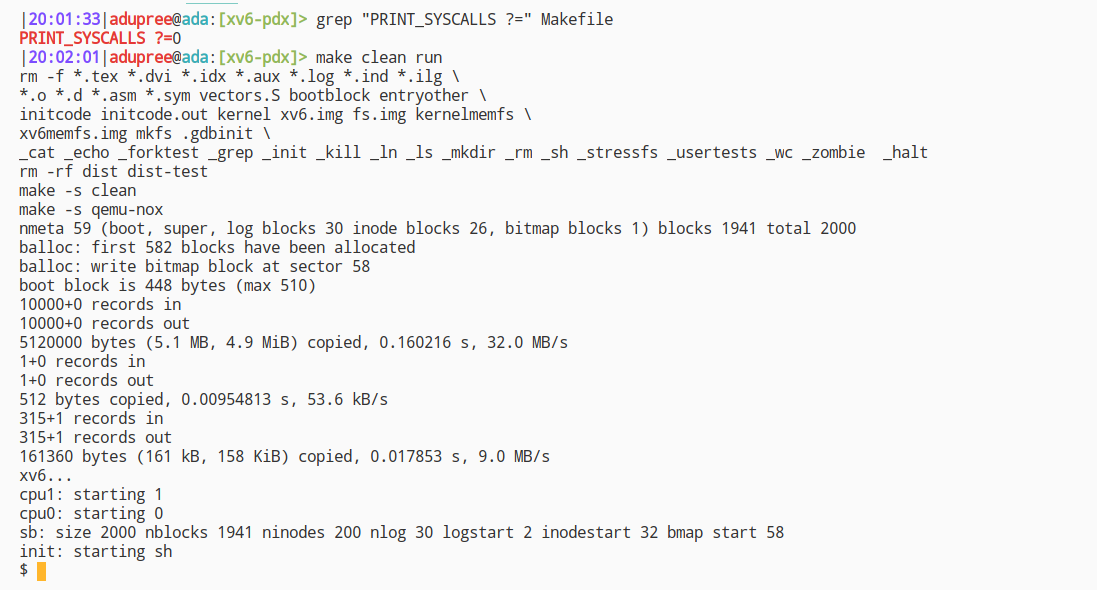
\includegraphics[width=1\linewidth]{test1.png}
	\caption[img]{Compilation and boot with CS333\_PROJECT set to 0.}
	\label{fig:P1compileP0-1}
  \end{figure}

  The command \code{grep "CS333\_PROJECT ?=" Makefile} shows that the CS333\_PROJECT define is truly set to 0.
  The following command \code{make clean run} demonstrates that the code correctly compiles successfully boots. 
  Furthermore, the commands were executed within seconds of each other, indicating that
  tampering is not a possibility.

\pagebreak

  \noindent\textbf{Test Case:} \emph{With CS333\_PROJECT set to 2 in the Makefile}
  
  \noindent\textbf{Assertions:}
  \begin{enumerate}[]
  \item Code correctly compiles
  \item Kernel successfully boots
  \end{enumerate}  
  
  \noindent\textbf{Status:} \textcolor{ForestGreen}{\textbf{PASS}}
  
  \begin{figure}[h!]
	\centering
	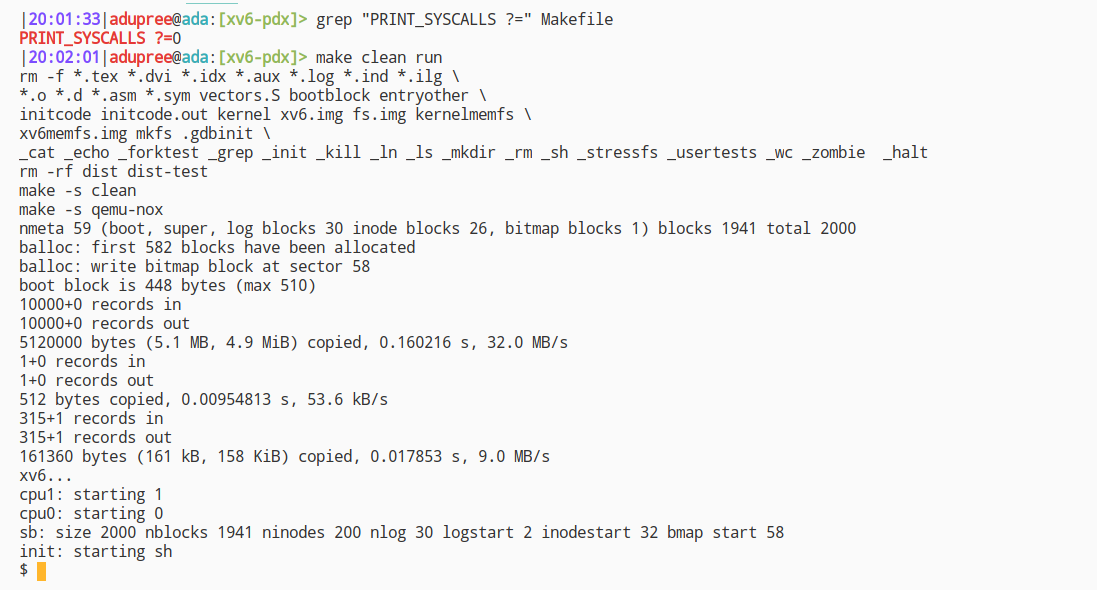
\includegraphics[width=1\linewidth]{test1.png}
	\caption[img]{Compilation and boot with CS333\_PROJECT set to 2, CS333\_P2 is defined.}
	\label{fig:P1compileP0-1}
  \end{figure}

  Lorem ipsum dolor sit amet, consectetur adipiscing elit, sed do eiusmod 
  tempor incididunt ut labore et dolore magna aliqua. Ut enim ad minim 
  veniam, quis nostrud exercitation ullamco laboris nisi ut aliquip ex ea 
  commodo consequat. Duis aute irure dolor in reprehenderit in voluptate 
  velit esse cillum dolore eu fugiat nulla pariatur. 

  \pagebreak

\ifdefined \LF
} % large print end
\fi

\end{document}